\section{Cipher Specifications}

\begin{frame}{Design rationale}
\begin{enumerate}
    \item KLEIN is collection of ciphers of different key length(64, 80, and 96) and fixed 64 bit block length.We shall denote these ciphers as KLEIN-64/80/96 based on their key lengths.
    \item We know that block cipher's security and implementation cost mainly depends on the key size and block size. Keeping in mind that lightweight ciphers are used in resource constrained machines like sensors, RFIDs, the block length is decided to be 64 bits as high-throughput is not expected in these devices as large block lengths and larger keys are unnecessary.
    \item As 64 bit key length might be little vulnerable if we consider attacks based on pre-computation and large storage capacities, it is suggested to use KLEIN-64 for message authentication codes and hash functions.
\end{enumerate}
\end{frame}

\begin{frame}{Optimal Platform}
\begin{enumerate}
    \item Generally light weight ciphers are optimized for hardware implementation as they are used in RFID tags and smart cards.
    \item But if a system can support the computation and memory requirements of the software implementation, the costs of manufacturing and maintenance will reduce drastically as we can simply update the implementation of the cipher by simply installing a software update.
    \item Software implementation is more flexible.
    \item Both the software and hardware implementations are lightweight.
\end{enumerate}
\end{frame}
\begin{frame}{Structure of KLEIN}
\begin{enumerate}
    \item KLEIN is made of Substitution-Permutation-Network(SPN) which is also used in popular ciphers like AES and PRESENT.
    \item By taking into the consideration of security margin and the asymmetric iteration we chose 12/16/20 rounds for KLIEN-64/80/96 respectively.
\end{enumerate}
\begin{algorithm}[H]
\SetAlgoLined
$sk^{1}\gets KEY$; \\
STATE $\gets$ PLAINTEXT;\\
\For{$i=1$ \KwTo $N_{R}$ }{
    $AddRoundKey(\text{STATE}, sk i );$\\
$SubN ibbles(\text{STATE});$ \\
$RotateN ibbles(\text{STATE});$ \\
$MixN ibbles(\text{STATE});$ \\
$sk_{i+1} = KeySchedule(sk_{i} , i);$ \\
 }
 CIPHERTEXT $\gets AddRoundKey(\text{STATE}, sk^{N_{R}+1} )$;
 \caption{KLEIN CIPHER}
\end{algorithm}
\end{frame}

\begin{frame}{Round Transformation}
\textbf{SubNibbles} \\
Before this step, the corresponding round key will be xor-ed with the input . The obtained resultant state is passed to subnibbles where the state is divided into 16 4-bit nibbles and given as input to the 4 x 4 Involutive permutation. \\ \\
Involutiveness of S-box is helpful to decrease the implementation costs of calculating its inverse and also the need of protect only one sbox instead of two(original and inverse) in other ciphers from side channel attacks.
\begin{center}\begin{math}
\begin{array}{|c|c|c|c|c|c|c|c|c|c|c|c|c|c|c|c|c|}
\hline
Input &0 &1 &2 &3 &4 &5 &6 &7 &8 &9 &A &B &C & D& E& F&  
\hline
Output &7 &4 &A &9 &1 &F &B &0 &C &3 &2 &6 &8 &E &D &5 & 
\hline
\end{array}
\end{math}
\end{center}
\end{frame}

\begin{frame}
It also satisfies following properties: \\
\begin{enumerate}
\item  It should not contain any fixed points i.e S(x)$\neq$x, where  $x \in \mathbb{F}^{4}_{2} $.
\item For any non-zero input diff($\Delta_{I}$) and output diff($\Delta_{O}$) that belong to  $\mathbb{F}^{4}_{2} $, It should follow:
$$ \#\{x \in \mathbb{F}^{4}_{2} | S(x) \oplus S(x \oplus \Delta_{I} ) = \Delta_{O} \} \leq 4$$.
Furthermore, if $wt(\Delta_{I} ) = wt(\Delta{O} )=1$, where $wt(X)=\sum_{i}X_{i}\;$($X_{i}$ is ith bit of X) , we have
$$\#\{x \in \mathbb{F}^{4}_{2} |S(x) \oplus S(x \oplus \Delta_{I} ) = \Delta_{O} \} \leq 2$$.
\end{enumerate}
\end{frame}

\begin{frame}
\textbf{Rotate Nibbles}
\begin{enumerate}
	
	\item Assume at the ith round state is $ b_{0} b_{1} b_{2} b_{3} b_{4} b_{5} b_{6} b_{7} b_{8} b_{9} b_{10} b_{11} b_{12} b_{13} b_{14} b_{15} $ where $b_{i}$ is a nibble. The rotate nibble step involves left circular shift of two bytes of this state i.e after the rotate nibbles step our state becomes $   b_{4} b_{5} b_{6} b_{7} b_{8} b_{9} b_{10} b_{11} b_{12} b_{13} b_{14} b_{15} b_{0} b_{1} b_{2} b_{3} $ 
\end{enumerate}
\end{frame}

\begin{frame}
	\textbf{Mix nibbles}
\begin{enumerate}

	\item Let the current state be $c_{0} c_{1} c_{2} c_{3} c_{4} c_{5} c_{6} c_{7} c_{8} c_{9} c_{10} c_{11} c_{12} c_{13} c_{14} c_{15}$\\
	
	\item This state is divided into two parts \\
	$ c_{0} c_{1} c_{2} c_{3} c_{4} c_{5} c_{6} c_{7} $ and $c_{8} c_{9} c_{10} c_{11} c_{12} c_{13} c_{14} c_{15}$ \\
	
	\item Each two nibble pair acts as a byte and each of the above part form a column. Then the multiplication process is same as that of one column of AES.
\end{enumerate}

\end{frame}	

\begin{frame}
	$\begin{bmatrix}
	s^{i+1}_{0} | s^{i+1}_{1}\\
	s^{i+1}_{2} | s^{i+1}_{3}\\
	s^{i+1}_{4} | s^{i+1}_{5}\\
	s^{i+1}_{6} | s^{i+1}_{7}
	\end{bmatrix}=
	\begin{bmatrix}
	2&3&1&1\\
	1&2&3&1\\
	1&1&2&3\\
	3&1&1&2
	\end{bmatrix}
	\begin{bmatrix}
	c_{0}|c_{1}\\
	c_{2}|c_{3}\\
	c_{4}|c_{5}\\
	c_{6}|c_{7}
	\end{bmatrix}  $ ,
	$\begin{bmatrix}
	s^{i+1}_{8} | s^{i+1}_{9}\\
	s^{i+1}_{10} | s^{i+1}_{11}\\
	s^{i+1}_{12} | s^{i+1}_{13}\\
	s^{i+1}_{14} | s^{i+1}_{15}
	\end{bmatrix}=
	\begin{bmatrix}
	2&3&1&1\\
	1&2&3&1\\
	1&1&2&3\\
	3&1&1&2
	\end{bmatrix}
	\begin{bmatrix}
	c_{8}|c_{9}\\
	c_{10}|c_{11}\\
	c_{12}|c_{13}\\
	c_{14}|c_{15}
	\end{bmatrix}  $\\ \\
	Thus we obtain the next state 
	$ s^{i+1}_{0}  s^{i+1}_{1}
	s^{i+1}_{2}  s^{i+1}_{3}
	s^{i+1}_{4}  s^{i+1}_{5}
	s^{i+1}_{6}  s^{i+1}_{7}
	s^{i+1}_{8}  s^{i+1}_{9}
	s^{i+1}_{10}  s^{i+1}_{11}
	s^{i+1}_{12}  s^{i+1}_{13}
	s^{i+1}_{14}  s^{i+1}_{15} $
\end{frame}
	
\begin{frame}{Key Schedule}

\begin{itemize}
	
	\item The first subkey $sk_{0}$ is same as the master key \\
	$sk_{0}$=$mk$.Each of the subsequent $sk_{i+1}$ will be derived from $sk_{i}$ as follows - \\
	
	\item Denote $sk_{i}$ as a tuple of bytes - (x0 x1 x2 x3 x4 x5 x6 x7) \\
	Divide the tuple into two equal parts and call them a and b 
	
	a - ($ x_{0}$ $x_{1}$ $x_{2}$ $x_{3}$) \\
	b - ($x_{4}$ $x_{5}$ $x_{6}$ $x_{7}$) \\
	
	\item Now Perform one byte left circular shift to both a and b
	
	$a'$ = ($x_{1}$ $x_{2}$ $x_{3}$ $x_{0}$) \\
	$b'$  = ($x_{7}$ $x_{4}$ $x_{5}$ $x_{6}$) \\
\end{itemize}
\end{frame}
\begin{frame}
\begin{itemize}

	\item Swap $a'$ and $b'$  i.e $a''$ = $b'$  and b''=$a'$ \\
	
	\item Now let $a''$ = ($y_{0}$ $y_{1}$ $y_{2}$ $y_{3}$) \\
	and $b''$ = ($z_{0}$ $z_{1}$ $z_{2}$ $z_{3}$) \\
	
	We will Xor the round counter i with 3rd byte of $a''$ and pass 2nd and 3rd byte of $b''$ through the KLIEN S-BOX and then $a''$$||$$b''$ will become the next subkey \\
	$sk_{i+1}$ = (y0 y1 $ y2 \oplus R_i $ y3 z0 Sbox(z1) Sbox(z2) z4)\\
\end{itemize}
\end{frame}
\begin{frame}
\begin{figure}[h]
    \centering
    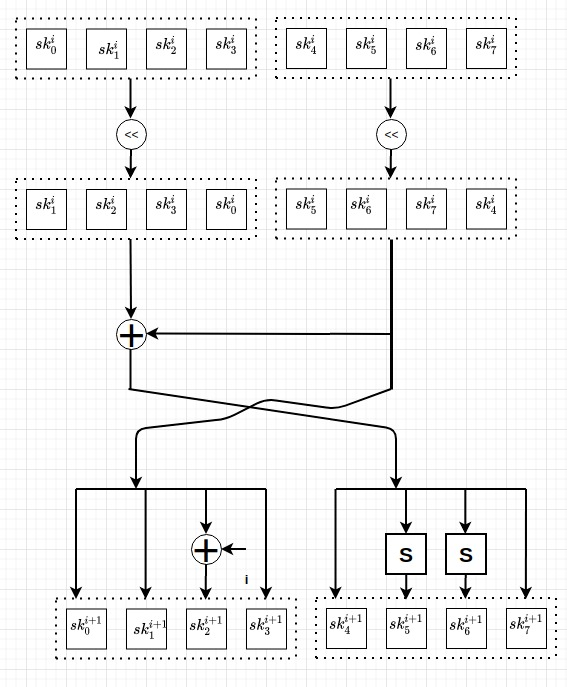
\includegraphics[width=6cm, hieght= 8cm, keepaspectratio]{images/key_schedule.jpeg}
    \caption{Key Schedule}
    \label{fig:key schedule}
\end{figure}
\end{frame}
\begin{frame}{Overview of KLEIN Cipher}
    \begin{figure}
    \centering
    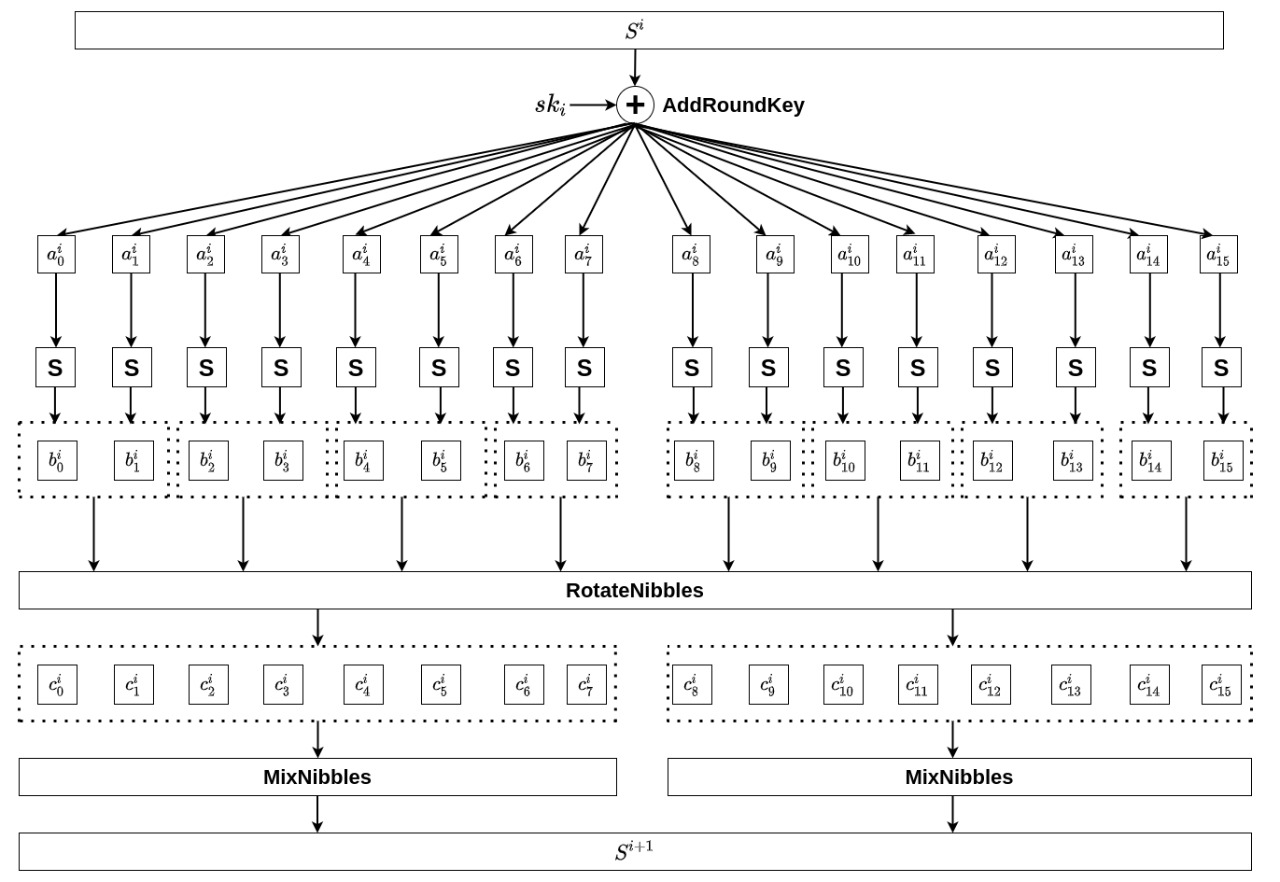
\includegraphics[width=8cm, hieght= 10cm, keepaspectratio]{images/klein_cipher.jpeg}
    \caption{KLEIN cipher}
    \label{fig:overview}
\end{figure}
\end{frame}

